\documentclass[a4paper]{article}


\usepackage[utf8]{inputenc}
\usepackage{graphicx}
\usepackage{natbib}

\title{Práctica Latex: Gatos}
\author{Álvaro Sáncez Pinedo y Jorge Zaragoza Garriós}
\date{ 5 de Noviembre de 2021}



\begin{document}
\maketitle


\pagebreak



\section{Introducción}

El nombre actual en muchas lenguas proviene del latín vulgar catus. Irónicamente, catus aludía a los gatos salvajes, mientras que los gatos domésticos, en latín, eran llamados felis. \\

Como resultado de mutaciones genéticas, cruzamiento y selección artificial, hay numerosas razas. Algunas, como la raza sphynx o la peterbald están desprovistas de pelo; otras carecen de cola, como los gatos de la raza manx, y algunas tienen coloraciones atípicas, como los llamados gatos azules. \\

Gato acostado al revés
El gato se comunica a través de vocalizaciones. Las más populares son su característico maullido y el ronroneo, pero puede aullar, gemir, gruñir y bufar.Los Gatos desarrollaron el maullido con la única finalidad de poder comunicarse con el ser humano. Además, adopta poses o expresiones que informan, a sus congéneres, sus enemigos o sus cuidadores, de su ánimo o sus intenciones.\\

Junto con el perro, es el animal doméstico más popular, como mascota, como ayuda en la lucha contra roedores o ambas cosas.
\\


\begin{figure}[h!]
\centering
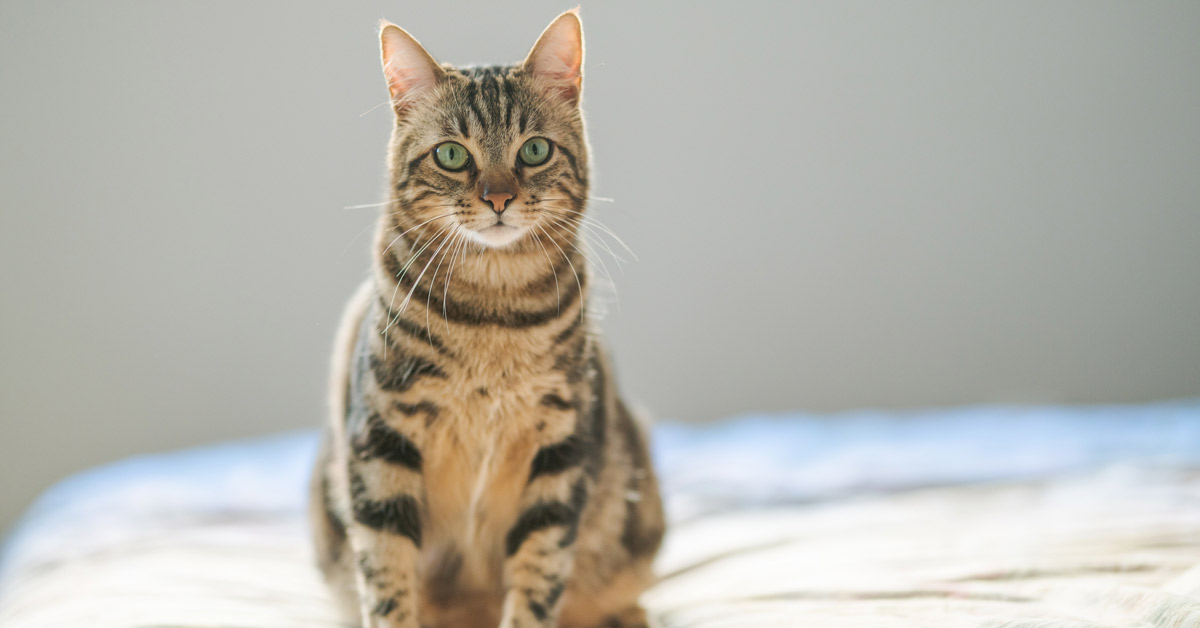
\includegraphics[scale=0.3]{gato.jpg}
\caption{Gato}
\label{fig:Gato1}
\end{figure}

\pagebreak




\section{Características}

Generalmente pesan entre 2,5 y 7 kg; sin embargo, algunas razas como el Ragdoll y el Maine Coon pueden exceder los 11,3 kilogramos. Han existido casos que superaron los 23 kg de peso debido a la sobrealimentación. El sobrepeso es perjudicial para el animal y debe ser evitado a través de una dieta equilibrada y ejercicio físico, especialmente en aquellos ejemplares exclusivamente hogareños.\\


Los gatos domésticos machos tienen una esperanza de vida de entre doce y catorce años, mientras que las hembras suelen vivir uno o dos años más. El ejemplo más longevo del que se tiene registro vivió treinta y ocho años. Tienden a vivir más tiempo si se les restringe la salida al exterior (disminuye el riesgo de lesiones producidas por peleas o accidentes y la exposición a enfermedades) y si se los esteriliza (reduce el riesgo de cáncer testicular o de ovarios). \\


Las hembras esterilizadas con anterioridad a su primer celo, tienen menos posibilidades de sufrir cáncer de mama. Los gatos callejeros que viven en entornos urbanos con frecuencia viven sólo dos años, o menos. Mantenidos en colonias pueden vivir muchos más años.
\\


\begin{table}[htbp]
\center
\caption{Características de los gatos}
\begin{tabular}{lccc}
\hline
Pelaje: & Monocolor & Bicolor & Tricolor\\
Temperatura: & 38.6º & 101.5 °F & 311.75 K\\
Comunicación: & Ronroneo & Maullidos & Gruñidos \\
\hline
\label{tabla1}
\end{tabular}
\end{table}

\begin{figure}[h!]
\centering
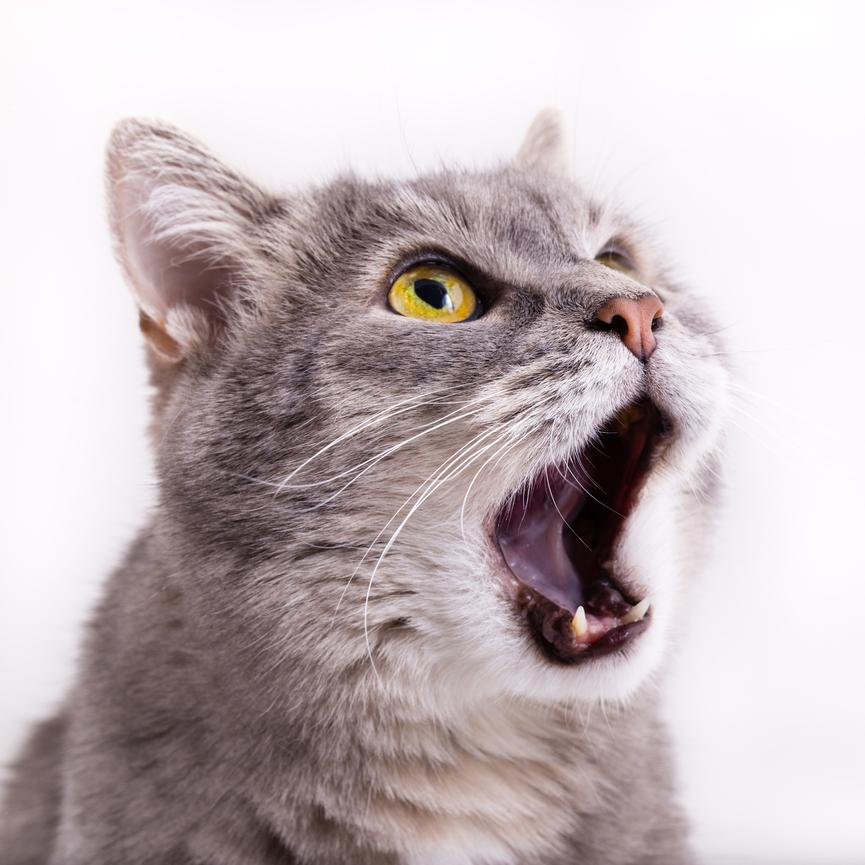
\includegraphics[scale=0.3]{gato2.jpg}
\caption{Gato Maullando}
\label{fig:Gato2}
\end{figure}












\pagebreak



\section{Dieta y caza}

En relación a su tamaño, los gatos domésticos son depredadores muy eficaces. Pueden emboscar y abalanzarse sobre distintos vertebrados usando tácticas similares a los leopardos, pumas, y tigres; es entonces cuando asestan la mordida letal con sus largos dientes caninos que rompen la médula espinal de la víctima, o la asfixia comprimiendo su tráquea. \\

Puede cazar y comer cerca de cien especies pero la mayoría de los grandes felinos carecen de tanta diversidad de especies para cazar. Sin embargo, teóricamente, los grandes felinos también pueden cazar las mismas especies que el gato, pero no lo hacen frecuentemente debido al contenido nutricional relativamente bajo que proveen estos animales. Una excepción es el leopardo y el lince ibérico, quienes usualmente cazan conejos y otros animales pequeños.\\

Los ejemplares bien alimentados pueden cazar y matar aves, ratones, ratas, lagartos y otros pequeños animales en las inmediaciones, para luego mostrar el trofeo de caza a sus dueños. El motivo por el cual lo hacen no está totalmente claro, pero se cree que esta acción está relacionada con los comportamientos de creación de lazos afectivos. \\

Es probable que esperen ser elogiados por su contribución simbólica al grupo. Se sabe que, en la vida salvaje, incluso un macho puede compartir su caza con miembros de su familia. El obsequio de piezas por parte de un animal bien alimentado puede ser usual, e interpretarse como un gesto de cariño y familiaridad.\\


\begin{table}[htbp]
\center
\caption{Características de los gatos}
\begin{tabular}{lccc}
\hline
Dieta: & Aves & Roedores & Lagartos\\
Método de Caza: & Rotula de médula & Asfixia & Hemorragia\\
\hline
\label{tabla2}
\end{tabular}
\end{table}

\begin{figure}[h!]
\centering
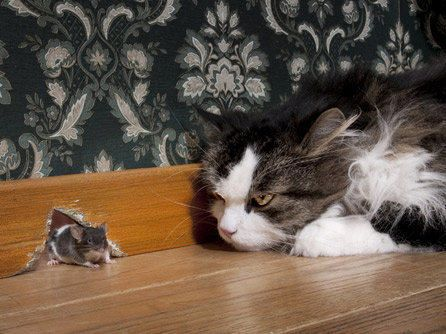
\includegraphics[scale=0.5]{gato3.jpg}
\caption{Gato cazando}
\label{fig:Gato3}
\end{figure}






\pagebreak


\section{El gato en la cultura popular}

Por su agilidad y fortaleza, y por su habilidad de caer sobre sus patas, se dice popularmente que tienen siete vidas, nueve en el mundo anglosajón, en ambos casos un número considerado de la buena suerte.\\

Por cuestiones culturales, en Occidente no se acostumbra a comer gatos. Este hecho, la ingesta de carne de gatos, perros u otros animales de compañía, suele causar repulsión entre la población. No obstante la expresión "dar gato por liebre" proviene de la sospecha de que los venteros, cuando no tenían liebre o conejo, servían carne de gato.\\

Durante el Siglo de Oro se usaban bolsas hechas de piel de gato para guardar el dinero, que acabarían llamándose "gatos". De ahí vendría la expresión "aquí hay gato encerrado", con el significado de un tesoro o secreto oculto a la mirada.\\

Debido a su carácter nocturno, y a que en la oscuridad es más difícil distinguir los colores, aparece la expresión "de noche todos los gatos son pardos" refiriéndose a la falta o poca relevancia de las diferencias entre lo que se menciona, o a la dificultad de distinguir dichas diferencias. Proviene de la referencia a que en la oscuridad de la noche, es más fácil ocultar los defectos de una mercancía.\\

\begin{figure}[h!]
\centering
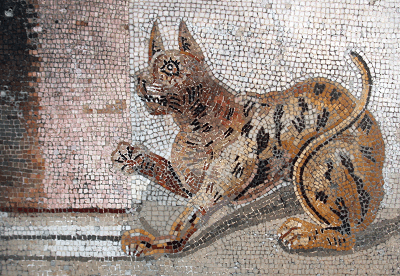
\includegraphics[scale=0.7]{gato4.png}
\caption{Gato en la cultura popular}
\label{fig:Gato4}
\end{figure}

\pagebreak















\end{document}